In this notebook, we're going to define and train a CycleGAN to read in
an image from a set \(X\) and transform it so that it looks as if it
belongs in set \(Y\). Specifically, we'll look at a set of images of
\href{https://en.wikipedia.org/wiki/Yosemite_National_Park}{Yosemite
national park} taken either during the summer of winter. The seasons are
our two domains!

\begin{quote}
The objective will be to train generators that learn to transform an
image from domain \(X\) into an image that looks like it came from
domain \(Y\) (and vice versa).
\end{quote}
Some examples of image data in both sets are pictured below.
\subsubsection{Unpaired Training Data}

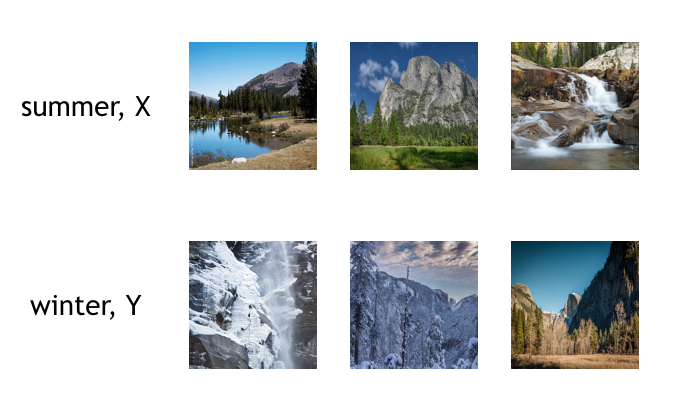
\includegraphics[width=1\linewidth]{img//genAdvNet//image2image/XY_season_images.png}

These images do not come with labels, but CycleGANs give us a way to
learn the mapping between one image domain and another using an
\textbf{unsupervised} approach. A CycleGAN is designed for
image-to-image translation and it learns from unpaired training data.
This means that in order to train a generator to translate images from
domain \(X\) to domain \(Y\), we do not have to have exact
correspondences between individual images in those domains. For example,
in \href{https://arxiv.org/abs/1703.10593}{the paper that introduced
CycleGANs}, the authors are able to translate between images of horses
and zebras, even though there are no images of a zebra in exactly the
same position as a horse or with exactly the same background, etc. Thus,
CycleGANs enable learning a mapping from one domain \(X\) to another
domain \(Y\) without having to find perfectly-matched, training pairs!

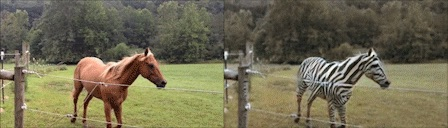
\includegraphics[width=1\linewidth]{img//genAdvNet//image2image/horse2zebra.jpg}

\subsubsection{CycleGAN and Exercises Structure}

A CycleGAN is made of two types of networks: \textbf{discriminators, and
generators}. In this example, the discriminators are responsible for
classifying images as real or fake (for both \(X\) and \(Y\) kinds of
images). The generators are responsible for generating convincing, fake
images for both kinds of images.

To successfully train a cycle gan, we need to do the following:

\begin{quote}
\begin{enumerate}
\item You'll load in the image data using PyTorch's DataLoader class to efficiently read in images from a specified directory.
\item \textbf{Then, you'll be tasked with defining the CycleGAN architecture according to provided specifications. You'll define the generator models and implement the different loss functions.}
\item You'll complete the training cycle by calculating the adversarial and cycle consistency losses for the generator and discriminator network and completing a number of training epochs. \emph{It's suggested that you enable GPU usage for training.}
\item Finally, you'll evaluate your model by looking at the loss over time and looking at sample, generated images.
\end{enumerate}
\end{quote}
\subsection{Define the Model}
A CycleGAN is made of two discriminator and two generator networks.
\subsection{Discriminators}
The discriminators, \(D_X\) and \(D_Y\), in this CycleGAN are
convolutional neural networks that see an image and attempt to classify
it as real or fake. In this case, real is indicated by an output close
to 1 and fake as close to 0. The discriminators have the following
architecture:

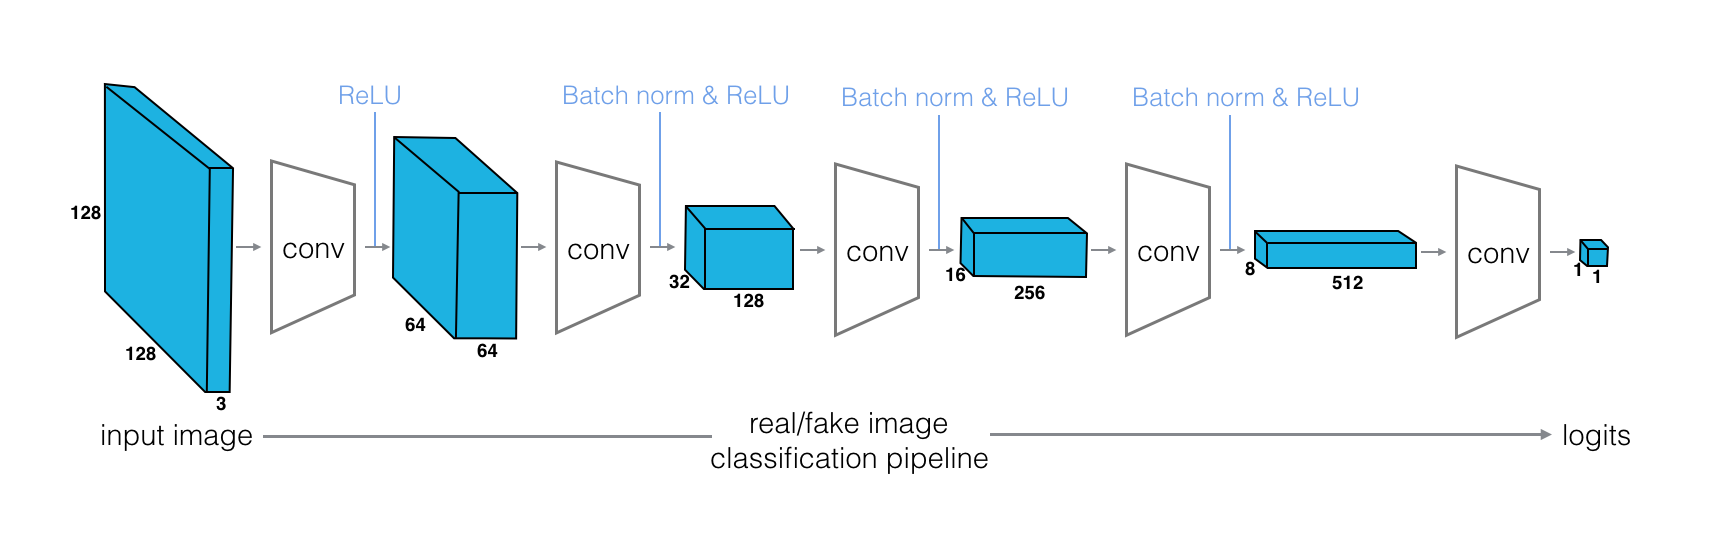
\includegraphics[width=1\linewidth]{img//genAdvNet//image2image/discriminator_layers.png}

This network sees a 128x128x3 image, and passes it through 5
convolutional layers that downsample the image by a factor of 2. The
first four convolutional layers have a BatchNorm and ReLu activation
function applied to their output, and the last acts as a classification
layer that outputs one value. \newline

\textbf{The discriminator architecture is not very different from the
DCGAN architecture and therefore we will focus on implementing the
generator only.}
\subsection{Generators}
The generators, \lstinline{G_XtoY} and
\lstinline{G_YtoX} (sometimes called F), are made of an
\textbf{encoder}, a conv net that is responsible for turning an image
into a smaller feature representation, and a \textbf{decoder}, a
\emph{transpose\_conv} net that is responsible for turning that
representation into an transformed image. These generators, one from
XtoY and one from YtoX, have the following architecture:

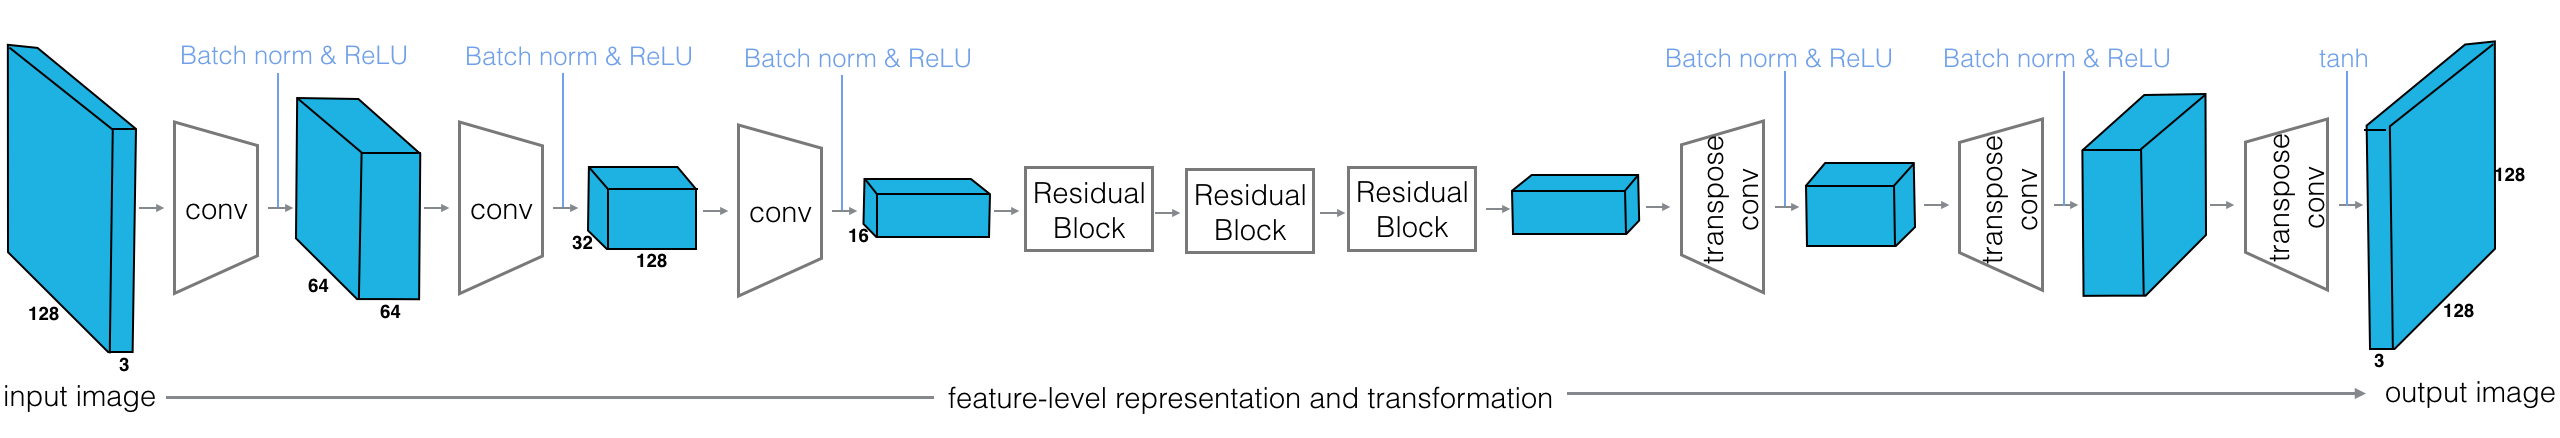
\includegraphics[width=1\linewidth]{img//genAdvNet//image2image/cyclegan_generator_ex.png}

This network sees a 128x128x3 image, compresses it into a feature
representation as it goes through three convolutional layers and reaches
a series of residual blocks. It goes through a few (typically 6 or more)
of these residual blocks, then it goes through three transpose
convolutional layers (sometimes called \emph{de-conv} layers) which
upsample the output of the resnet blocks and create a new image! \newline

Note that most of the convolutional and transpose-convolutional layers
have BatchNorm and ReLu functions applied to their outputs with the
exception of the final transpose convolutional layer, which has a
\lstinline{tanh} activation function applied to the
output. Also, the residual blocks are made of convolutional and batch
normalization layers, which we'll go over in more detail, next.
\subsubsection{Residual Block Class}
To define the generators, you're expected to define a
\lstinline{ResidualBlock} class which will help you
connect the encoder and decoder portions of the generators. You might be
wondering, what exactly is a Resnet block? It may sound familiar from
something like ResNet50 for image classification, pictured below.

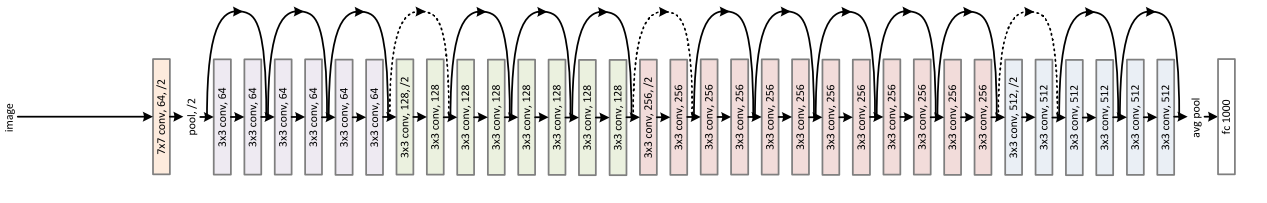
\includegraphics[width=1\linewidth]{img//genAdvNet//image2image/resnet_50.png}

ResNet blocks rely on connecting the output of one layer with the input
of an earlier layer. The motivation for this structure is as follows:
very deep neural networks can be difficult to train. Deeper networks are
more likely to have vanishing or exploding gradients and, therefore,
have trouble reaching convergence; batch normalization helps with this a
bit. However, during training, we often see that deep networks respond
with a kind of training degradation. Essentially, the training accuracy
stops improving and gets saturated at some point during training. In the
worst cases, deep models would see their training accuracy actually
worsen over time! \newline

One solution to this problem is to use \textbf{Resnet blocks} that allow
us to learn so-called \emph{residual functions} as they are applied to
layer inputs. You can read more about this proposed architecture in the
paper, \href{https://arxiv.org/pdf/1512.03385.pdf}{Deep Residual
Learning for Image Recognition} by Kaiming He et. al, and the below
image is from that paper.

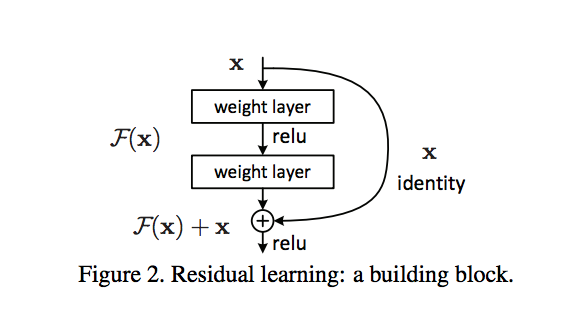
\includegraphics[width=0.5\linewidth]{img//genAdvNet//image2image/resnet_block.png}

\subsubsection{Residual Functions}
Usually, when we create a deep learning model, the model (several layers
with activations applied) is responsible for learning a mapping,
\(M\), from an input \(x\)
to an output \(y\).
\begin{quote}
    \(M(x) = y\) (Equation 1)
\end{quote}

Instead of learning a direct mapping from \(x\) to
\lstinline{y}, we can instead define a \textbf{residual function}
\begin{quote}
    \(F(x) = M(x) - x\)
\end{quote}

This looks at the difference between a mapping applied to x and the
original input, x. \(F(x)\) is, typically, two
convolutional layers + normalization layer and a ReLu in between. These
convolutional layers should have the same number of inputs as outputs.
This mapping can then be written as the following; a function of the
residual function and the input x. The addition step creates a kind of
loop that connects the input x to the output, y:
\begin{quote}
    \(M(x) = F(x) + x\) (Equation 2) or
\end{quote}
\begin{quote}
\(y = F(x) + x\) (Equation 3)
\end{quote}

\paragraph{Optimizing a Residual Function}
The idea is that it is easier to optimize this residual function
\(F(x)\)than it is to optimize the original
mapping \(M(x)\). Consider an example; what if we
want \(y = x\)? \newline

From our first, direct mapping equation, \textbf{Equation 1}, we could
set \(M(x) = x\) but it is easier to solve the
residual equation \(F(x) = 0\), which, when
plugged in to \textbf{Equation 3}, yields
\(y = x\).
\subsubsection{\texorpdfstring{Defining the \texttt{ResidualBlock} Class}{Defining the ResidualBlock Class}}

To define the \lstinline{ResidualBlock} class, we'll
define residual functions (a series of layers), apply them to an input x
and add them to that same input. This is defined just like any other
neural network, with an \lstinline{__init__} function
and the addition step in the \lstinline{forward} function. \newline

In our case, you'll want to define the residual block as: 
\begin{itemize}
    \item Two convolutional layers with the same size input and output
    \item Batch normalization applied to the outputs of the convolutional layers
    \item A ReLu function on the output of the \emph{first} convolutional layer
\end{itemize}

Then, in the \lstinline{forward} function, add the input x
to this residual block. Feel free to use the helper
\lstinline{conv} function from above to create this block.

\begin{lstlisting}[language=Python]
import torch
import torch.nn as nn

import tests
\end{lstlisting}

\begin{lstlisting}[language=Python]
class ConvBlock(nn.Module):
    """
    A convolutional block is made of 3 layers: Conv -> BatchNorm -> Activation.
    args:
    - in_channels: number of channels in the input to the conv layer
    - out_channels: number of filters in the conv layer
    - kernel_size: filter dimension of the conv layer
    - stride: stride of the conv layer
    - activation: whether to use an activation function or not
    """
    def __init__(self, 
                 in_channels: int, 
                 out_channels: int, 
                 kernel_size: int,
                 stride: int = 1,
                 activation: bool = True):
        super(ConvBlock, self).__init__()
        
        self.conv = nn.Conv2d(in_channels, out_channels, kernel_size, stride=stride, padding=1, bias=False)
        self.bn = nn.BatchNorm2d(out_channels)
        self.activation = activation
        if self.activation:
            self.act = nn.ReLU()
        
    def forward(self, x: torch.Tensor) -> torch.Tensor:
        x = self.conv(x)
        x = self.bn(x)
        if self.activation:
            x = self.act(x)
        return x
\end{lstlisting}

\begin{lstlisting}[language=Python]
# residual block class
class ResidualBlock(nn.Module):
    """Defines a residual block.
       This adds an input x to a convolutional layer (applied to x) with the same size input and output.
       These blocks allow a model to learn an effective transformation from one domain to another.
    """
    def __init__(self, conv_dim):
        super(ResidualBlock, self).__init__()
        # conv_dim = number of inputs
        # define two convolutional layers + batch normalization that will act as our residual function, F(x)
        # layers should have the same shape input as output; I suggest a kernel_size of 3
        self.conv_block1 = ConvBlock(in_channels=conv_dim, out_channels=conv_dim, kernel_size=3)
        self.conv_block2 = ConvBlock(in_channels=conv_dim, out_channels=conv_dim, kernel_size=3, activation=False)
        
    def forward(self, x):
        # apply a ReLu activation the outputs of the first layer
        # return a summed output, x + resnet_block(x)
        out_1 = self.conv_block1(x)
        out_2 = x + self.conv_block2(out_1)
        return out_2
\end{lstlisting}

\subsubsection{Transpose Convolutional Helper Function}

To define the generators, you're expected to use the above
\lstinline{conv} function,
\lstinline{ResidualBlock} class, and the below
\lstinline{deconv} helper function, which creates a
transpose convolutional layer + an optional batchnorm layer.

\begin{lstlisting}[language=Python]
class DeconvBlock(nn.Module):
    """
    A "de-convolutional" block is made of 3 layers: ConvTranspose -> BatchNorm -> Activation.
    args:
    - in_channels: number of channels in the input to the conv layer
    - out_channels: number of filters in the conv layer
    - kernel_size: filter dimension of the conv layer
    - stride: stride of the conv layer
    - padding: padding of the conv layer
    - batch_norm: whether to use batch norm or not
    """
    def __init__(self, 
                 in_channels: int, 
                 out_channels: int, 
                 kernel_size: int, 
                 stride: int = 2,
                 padding: int = 1,
                 batch_norm: bool = True):
        super(DeconvBlock, self).__init__()
        self.deconv = nn.ConvTranspose2d(in_channels, out_channels, kernel_size, stride, padding, bias=False)
        self.batch_norm = batch_norm
        if self.batch_norm:
            self.bn = nn.BatchNorm2d(out_channels)
        self.activation = nn.ReLU()
        
    def forward(self, x: torch.Tensor) -> torch.Tensor:
        x = self.deconv(x)
        if self.batch_norm:
            x = self.bn(x)
        x = self.activation(x)
        return x
\end{lstlisting}

\subsection{Define the Generator Architecture}

\begin{itemize}
\item Complete the \lstinline{__init__} function with the specified 3 layer \textbf{encoder} convolutional net, a series of residual blocks (the number of which is given by \lstinline{n_res_blocks}), and then a 3 layer \textbf{decoder} transpose convolutional net.
\item Then complete the \lstinline{forward} function to define the forward behavior of the generators. Recall that the last layer has a \lstinline{tanh} activation function.
\end{itemize}

Both \(G_{XtoY}\) and \(G_{YtoX}\) have the same architecture, so we
only need to define one class, and later instantiate two generators.

\begin{lstlisting}[language=Python]
class CycleGenerator(nn.Module):
    
    def __init__(self, conv_dim: int = 64, n_res_blocks: int = 6):
        super(CycleGenerator, self).__init__()

        # 1. Define the encoder part of the generator
        
        # initial convolutional layer given, below
        self.conv1 = ConvBlock(3, conv_dim, 4, stride=2)
        self.conv2 = ConvBlock(conv_dim, conv_dim*2, 4, stride=2)
        self.conv3 = ConvBlock(conv_dim*2, conv_dim*4, 4, stride=2)

        # 2. Define the resnet part of the generator
        # Residual blocks
        self.res_layers = nn.ModuleList()
        for layer in range(n_res_blocks):
            self.res_layers.append(ResidualBlock(conv_dim*4))

        # 3. Define the decoder part of the generator
        # two transpose convolutional layers and a third that looks a lot like the initial conv layer
        self.deconv1 = DeconvBlock(conv_dim*4, conv_dim*2, 4)
        self.deconv2 = DeconvBlock(conv_dim*2, conv_dim, 4)
        # no batch norm on last layer
        self.deconv3 = nn.ConvTranspose2d(conv_dim, 3, 4, 2, 1, bias=False)
        
        self.final_act = nn.Tanh()
        
    def forward(self, x: torch.Tensor) -> torch.Tensor:
        """Given an image x, returns a transformed image."""
        # define feedforward behavior, applying activations as necessary
        out = self.conv1(x)
        out = self.conv2(out)
        out = self.conv3(out)
        
        for layer in self.res_layers:
            out = layer(out)
        
        out = self.deconv1(out)
        out = self.deconv2(out)
        # tanh applied to last layer
        out = self.deconv3(out)
        out = self.final_act(out)
        return out
\end{lstlisting}

\begin{lstlisting}[language=Python]
generator = CycleGenerator()
\end{lstlisting}

\begin{lstlisting}[language=Python]
def check_cycle_generator(generator: nn.Module):
    image = torch.randn(1, 3, 128, 128)
    output = generator(image)
    print(output.shape)
\end{lstlisting}

\begin{lstlisting}[language=Python]
tests.check_cycle_generator(generator)
\end{lstlisting}

\subsection{Discriminator and Generator Losses}
Computing the discriminator and the generator losses are key to getting a CycleGAN to train.

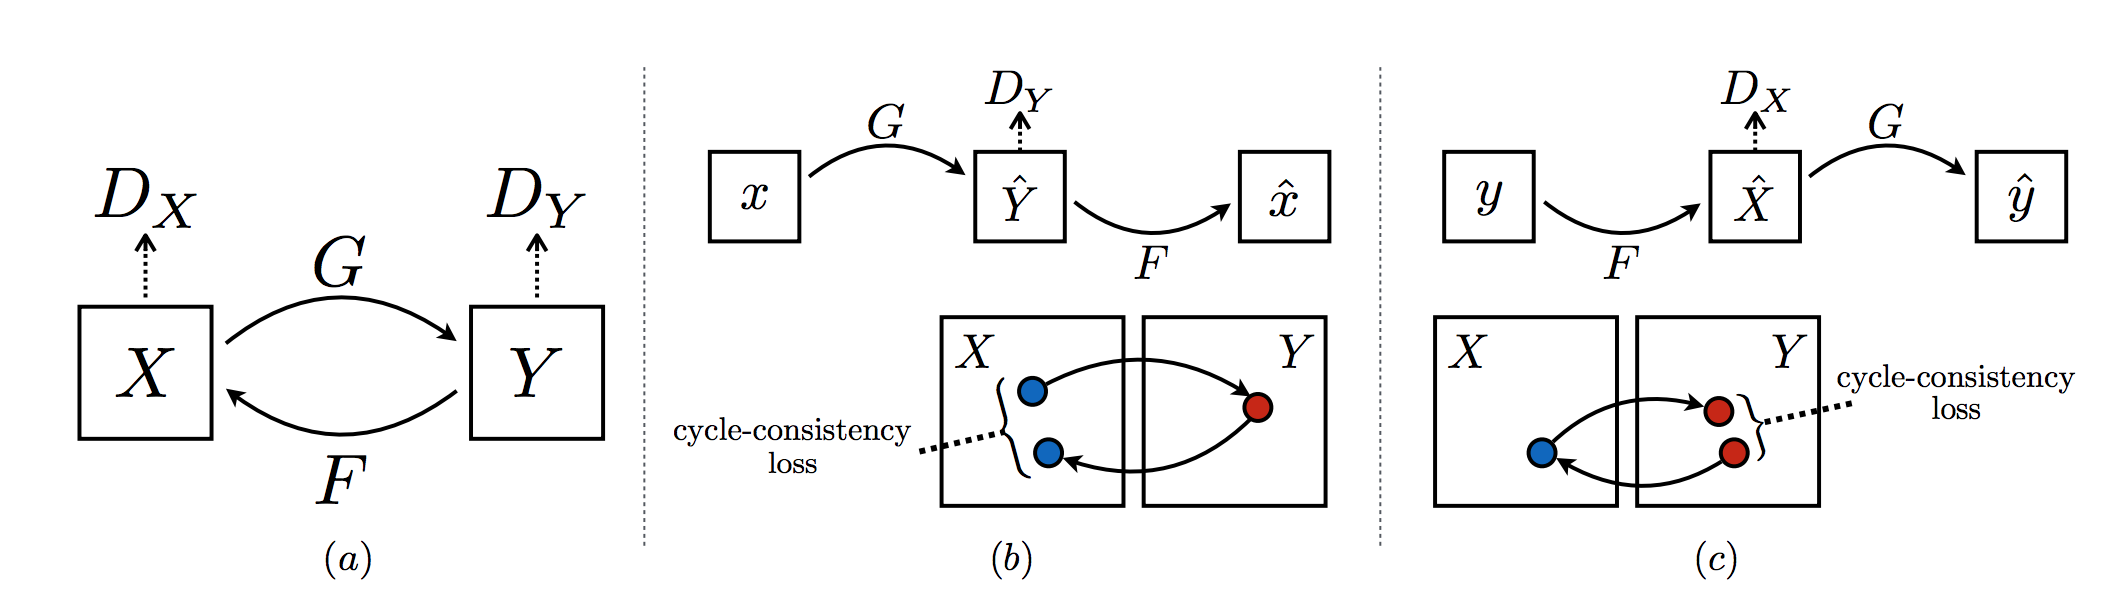
\includegraphics[width=1\linewidth]{img//genAdvNet//image2image/CycleGAN_loss.png}
\captionof{figure}{\textbf{Image from \href{https://arxiv.org/abs/1703.10593}{original paper} by Jun-Yan Zhu et. al.}}

\begin{itemize}
\item The CycleGAN contains two mapping functions \(G: X \rightarrow Y\) and \(F: Y \rightarrow X\), and associated adversarial discriminators \(D_Y\) and \(D_X\). \textbf{(a)} \(D_Y\) encourages \(G\) to translate \(X\) into outputs indistinguishable from domain \(Y\), and vice versa for \(D_X\) and \(F\).
\item To further regularize the mappings, we introduce two cycle consistency losses that capture the intuition that if we translate from one domain to the other and back again we should arrive at where we started. \textbf{(b)} Forward cycle-consistency loss and \textbf{(c)} backward cycle-consistency loss.
\end{itemize}
\subsection{Least Squares GANs}
We've seen that regular GANs treat the discriminator as a classifier
with the sigmoid cross entropy loss function. However, this loss
function may lead to the vanishing gradients problem during the learning
process. To overcome such a problem, we'll use a least squares loss
function for the discriminator. This structure is also referred to as a
least squares GAN or LSGAN, and you can
\href{https://arxiv.org/pdf/1611.04076.pdf}{read the original paper on
LSGANs, here}. The authors show that LSGANs are able to generate higher
quality images than regular GANs and that this loss type is a bit more
stable during training!
\subsubsection{Discriminator Losses}
The discriminator losses will be mean squared errors between the output
of the discriminator, given an image, and the target value, 0 or 1,
depending on whether it should classify that image as fake or real. For
example, for a \emph{real} image, \(x\), we can
train \(D_X\) by looking at how close it is to recognizing and image
\(x\) as real using the mean squared error:
\begin{lstlisting}
out_x = D_X(x)
real_err = torch.mean((out_x-1)**2)
\end{lstlisting}
\subsubsection{Generator Losses}
Calculating the generator losses will look somewhat similar to
calculating the discriminator loss; there will still be steps in which
you generate fake images that look like they belong to the set of \(X\)
images but are based on real images in set \(Y\), and vice versa. You'll
compute the ``real loss'' on those generated images by looking at the
output of the discriminator as it's applied to these \emph{fake} images;
this time, your generator aims to make the discriminator classify these
fake images as \emph{real} images.

\paragraph{Cycle Consistency Loss}

In addition to the adversarial losses, the generator loss terms will
also include the \textbf{cycle consistency loss}. This loss is a measure
of how good a reconstructed image is, when compared to an original
image. \newline

Say you have a fake, generated image, \lstinline{x_hat},
and a real image, \lstinline{y}. You can get a
reconstructed \lstinline{y_hat} by applying
\lstinline{G_XtoY(x_hat) = y_hat} and then check to see
if this reconstruction \lstinline{y_hat} and the orginal
image \lstinline{y} match. For this, we recommed
calculating the L1 loss, which is an absolute difference, between
reconstructed and real images. You may also choose to multiply this loss
by some weight value \lstinline{lambda_weight} to convey
its importance.

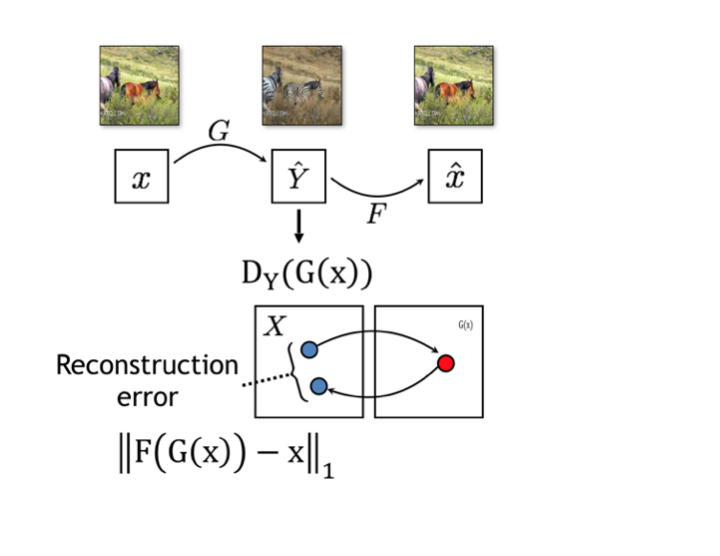
\includegraphics[width=1\linewidth]{img//genAdvNet//image2image/reconstruction_error.png}

The total generator loss will be the sum of the generator losses and the
forward and backward cycle consistency losses.

\subsubsection{Define Loss Functions}

To help us calculate the discriminator and gnerator losses during
training, let's define some helpful loss functions. Here, we'll define
three. 1. \lstinline{real_mse_loss} that looks at the
output of a discriminator and returns the error based on how close that
output is to being classified as real. This should be a mean squared
error. 2. \lstinline{fake_mse_loss} that looks at the
output of a discriminator and returns the error based on how close that
output is to being classified as fake. This should be a mean squared
error. 3. \lstinline{cycle_consistency_loss} that looks
at a set of real image and a set of reconstructed/generated images, and
returns the mean absolute error between them. This has a
\lstinline{lambda_weight} parameter that will weight the
mean absolute error in a batch.

It's recommended that you take a
\href{https://arxiv.org/pdf/1703.10593.pdf}{look at the original,
CycleGAN paper} to get a starting value for
\lstinline{lambda_weight}.

\begin{lstlisting}[language=Python]
def real_mse_loss(D_out: torch.Tensor) -> torch.Tensor:
    # how close is the produced output from being "real"?
    return torch.mean((D_out-1)**2)

def fake_mse_loss(D_out: torch.Tensor) -> torch.Tensor:
    # how close is the produced output from being "false"?
    return torch.mean(D_out**2)

def cycle_consistency_loss(real_im: torch.Tensor, 
                           reconstructed_im: torch.Tensor, 
                           lambda_weight: torch.Tensor) -> torch.Tensor:
    # calculate reconstruction loss 
    # as absolute value difference between the real and reconstructed images
    reconstr_loss = torch.mean(torch.abs(real_im - reconstructed_im))
    # return weighted loss
    return lambda_weight * reconstr_loss    
\end{lstlisting}

\begin{lstlisting}[language=Python]
tests.check_losses(real_mse_loss, fake_mse_loss, cycle_consistency_loss)
\end{lstlisting}
